% !TeX root = .
% Paper section: per-packet vs per-flow load balancing evaluation on a
% two-leaf / two-spine VXLAN fabric emulated with tofino-model.
% Requires: booktabs (tables), multirow (tables), graphicx (figure),
% amsmath (optional). Numbers come from leaf-spine/results.md
% (rounds R1 m8e2, R2 m16e3, R3 m32e4, 2026-09-28); the figure is
% regenerated with leaf-spine/paper_figure.py.

\section{Evaluation}
\label{sec:evaluation}

\subsection{Experimental Topology}
\label{sec:topology}

We evaluate on a two-leaf, two-spine Clos fabric emulated with the Intel
Tofino behavioral model (tofino-model, BF SDE~9.13.3), shown in
Figure~\ref{fig:topology}. Leaf~1 executes the P4 program under test (TNA
architecture) and performs the load-balancing decision; Leaf~2 is a remote
node terminating the tenant subnets.

\textbf{Hosts.} Eight tenants hang off Leaf~1 (\texttt{h1}--\texttt{h8},
10.100.1.11--18, Linux network namespaces over veth pairs) and eight off
Leaf~2 (\texttt{h9}--\texttt{h16}, 10.100.2.21--28). The host MTU is
1400~B to fit the VXLAN overlay.

\textbf{Spines.} The two spines are VXLAN tunnels from Leaf~1 (VNI~101 to
spine~1 via egress port~6; VNI~102 to spine~2 via egress port~7). An ECMP
group of the two spine next-hops is programmed at Leaf~1; all cross-leaf
traffic is subject to the load-balancing decision under study.

\textbf{Load balancer.} The same P4 source is compiled in two
configurations: \emph{Classic ECMP} hashes the 5-tuple only, pinning each
flow to one spine for its lifetime; \emph{MixHash} augments the selector
key with two per-packet header fields (RoCE BTH \texttt{psn[15:0]} and
IPv4 \texttt{identification}), so the forwarding choice is re-evaluated
every packet. Both binaries carry identical measurement logic.

\subsection{Traffic Generation and Measurement}
\label{sec:methodology}

\textbf{In-switch measurement.} Instead of out-of-band capture, the P4
program itself maintains per-flow, per-spine packet counters in two
4096-entry stateful-ALU registers indexed by a 12-bit hash of the inner
source and destination addresses. After the ECMP decision, each packet
increments the counter of the spine it was actually routed to. Because the
logging code lives outside the \texttt{CLASSIC\_ECMP} conditional, both
builds are instrumented identically; the only difference between the two
configurations under test is the hashing input.

\textbf{Workloads.} We run three increasingly heavy incast-style rounds.
In each, elephant flows (768~KB TCP, \texttt{dd~|~nc}) start at $t=0$ and
mice flows (64~KB TCP) at $t=+2$~s, with destinations shuffled so that
every Leaf-2 host receives an equal share. Table~\ref{tab:workloads}
summarizes the rounds. Per-flow completion time (FCT) is timestamped at
the senders; receiver-side byte counts verify full delivery in every run
(all mice 65{,}536~B, all elephants 786{,}432~B). We report per-flow
\emph{spine skew}, $|s_1 - s_2| / (s_1 + s_2)$, where 0 denotes perfect
spreading across spines and 1 complete pinning, together with the
aggregate spine traffic split.

\begin{table}[t]
  \centering
  \caption{Evaluation workloads. Elephants start at $t=0$, mice at $t=+2$~s; destinations shuffled so every destination host receives an equal number of mice.}
  \label{tab:workloads}
  \begin{tabular}{lrrrr}
    \toprule
    Round & Elephants & Mice & Concurrent flows & Total volume \\
    \midrule
    R1 & 2 & 8\,(\,1 per sender\,)  & 10 & 2\,MB \\
    R2 & 3 & 16\,(\,2 per sender\,) & 19 & 3.3\,MB \\
    R3 & 4 & 32\,(\,4 per sender\,) & 36 & 5\,MB \\
    \bottomrule
  \end{tabular}
\end{table}

\subsection{Results}
\label{sec:results}

Figure~\ref{fig:comparison} visualizes both the dispersion and the FCT
results; Tables~\ref{tab:dispersion} and~\ref{tab:fct} give the exact
values.

\begin{figure}[t]
  \centering
  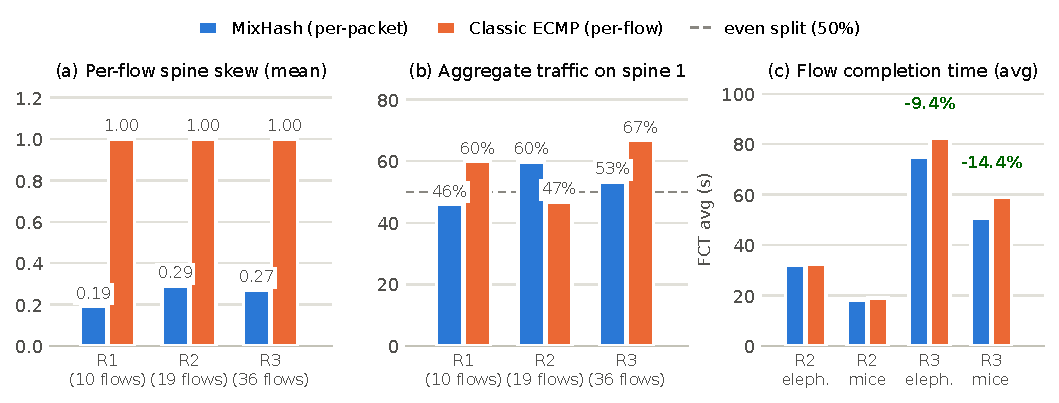
\includegraphics[width=\linewidth]{dispersion_fct}
  \caption{MixHash vs.\ Classic ECMP across the three rounds.
    (a)~Mean per-flow spine skew: Classic pins every flow (1.00);
    MixHash spreads each flow packet-by-packet ($\le 0.29$).
    (b)~Aggregate share of forwarded traffic on spine~1 against the even
    50\% line: Classic's balance is a hash lottery (46.7\%--66.7\%);
    MixHash converges toward even as the flow count grows.
    (c)~Mean FCT: the modes tie while both spines are balanced (R2), but
    when Classic's draw imbalances the fabric 2:1 (R3), MixHash finishes
    elephants 9.4\% and mice 14.4\% sooner.}
  \label{fig:comparison}
\end{figure}

\textbf{Spine dispersion.} Table~\ref{tab:dispersion} summarizes
forwarding balance across rounds.

\begin{table}[t]
  \centering
  \caption{Spine forwarding balance per round. Skew is
    $|s_1-s_2|/(s_1+s_2)$ per flow (0\,=\,perfectly spread,
    1\,=\,pinned); aggregate is the spines' share of forwarded packets.}
  \label{tab:dispersion}
  \begin{tabular}{llrr}
    \toprule
     &  & MixHash & Classic ECMP \\
    \midrule
    \multirow{2}{*}{R1}
      & per-flow skew (mean, range) & 0.19 (0.02--0.42) & 1.00 (10/10 pinned) \\
      & aggregate sp1 share         & 46.0\%            & 60.0\% \\
    \addlinespace
    \multirow{2}{*}{R2}
      & per-flow skew (mean, range) & 0.29 (0.04--0.61) & 1.00 (19/19 pinned) \\
      & aggregate sp1 share         & 59.8\%            & 46.7\% \\
    \addlinespace
    \multirow{2}{*}{R3}
      & per-flow skew (mean, range) & 0.27 (0.02--0.61) & 1.00 (36/36 pinned) \\
      & aggregate sp1 share         & 53.2\%            & 66.7\% \\
    \bottomrule
  \end{tabular}
\end{table}

Classic ECMP pins every flow in all rounds by construction. Its
\emph{aggregate} balance is a hash lottery: it happened to land near even
with 19 flows (46.7\%), but with 36 flows the draw placed 24 flows on one
spine, leaving it carrying $2\times$ the traffic of the other (66.7\%).
MixHash, in contrast, spreads every flow packet-by-packet: per-flow skew
never exceeds 0.61, and its aggregate share converged toward even as the
flow count grew (59.8\% $\rightarrow$ 53.2\% at 36 flows), since per-flow
hash biases average out across many flows.

\textbf{Flow completion time.} Table~\ref{tab:fct} reports FCT.

\begin{table}[t]
  \centering
  \caption{Flow completion time (ms). $\Delta$ is MixHash's improvement
    over Classic ECMP.}
  \label{tab:fct}
  \begin{tabular}{llrrr}
    \toprule
    Round & Metric & MixHash & Classic & $\Delta$ \\
    \midrule
    \multirow{2}{*}{R2}
      & elephant avg / max & 31{,}807 / 32{,}372 & 32{,}436 / 33{,}383 & $-2$\% / $-3$\% \\
      & mice avg / max      & 18{,}070 / 32{,}713 & 18{,}916 / 33{,}750 & $-4.5$\% / $-3$\% \\
    \addlinespace
    \multirow{2}{*}{R3}
      & elephant avg / max & 74{,}676 / 75{,}460 & 82{,}451 / 82{,}898 & $\mathbf{-9.4}$\% / $-9$\% \\
      & mice avg / max      & 50{,}403 / 73{,}558 & 58{,}886 / 86{,}428 & $\mathbf{-14.4}$\% / $\mathbf{-14.9}$\% \\
    \bottomrule
  \end{tabular}
\end{table}

At 19 concurrent flows the two modes are statistically indistinguishable,
while at 36 flows MixHash wins every metric with a double-digit margin on
mice. The trend tracks the dispersion data: once Classic's hash draw
concentrated two-thirds of the traffic on one spine, the overloaded path
became the bottleneck, whereas MixHash's even split kept both spines in
the fast regime. R1 showed identical FCT between modes with near-even
classic hashing, consistent with balance, not the hash scheme itself,
driving completion time.

\subsection{Discussion}
\label{sec:discussion}

\textbf{Dispersion is the controlled, reproducible win.} Per-flow skew is
1.00 for every classic flow in every round, versus $\le 0.61$ for MixHash
--- a deterministic, structural result. Aggregate balance under classic
ECMP is luck of the draw and degrades non-gracefully as flow count grows
(60\% $\rightarrow$ 46.7\% $\rightarrow$ 66.7\% across rounds);
MixHash's aggregate error shrank to 3.2\% at 36 flows.

\textbf{FCT penalty of imbalance emerges with scale.} When the classic
hash happened to balance (R1, R2), FCT parity followed; when it imbalanced
2:1 (R3), elephants slowed 9\% and mice 14--15\%. This is the causal chain
the per-packet design targets: hash collision $\rightarrow$ spine overload
$\rightarrow$ inflated FCT, with short, latency-sensitive mice hurt more
than elephants.

\textbf{Testbed caveats.} The behavioral model caps aggregate throughput
well below line rate ($\sim$0.5--1.4~Mbps effective here), so absolute
FCTs are dominated by model CPU scheduling --- e.g., mice FCT clusters by
sender host identically in both modes. The relative comparisons within a
round remain valid because both builds run the same binary logic,
measurement instrumentation, and traffic pattern; absolute latencies
should not be extrapolated to hardware.
